\documentclass{standalone}
\usepackage{tikz}
\usetikzlibrary{patterns, positioning}
\usepackage[sfdefault]{ClearSans} %% option 'sfdefault' activates Clear Sans as the default text font
\usepackage[T1]{fontenc}

\begin{document}
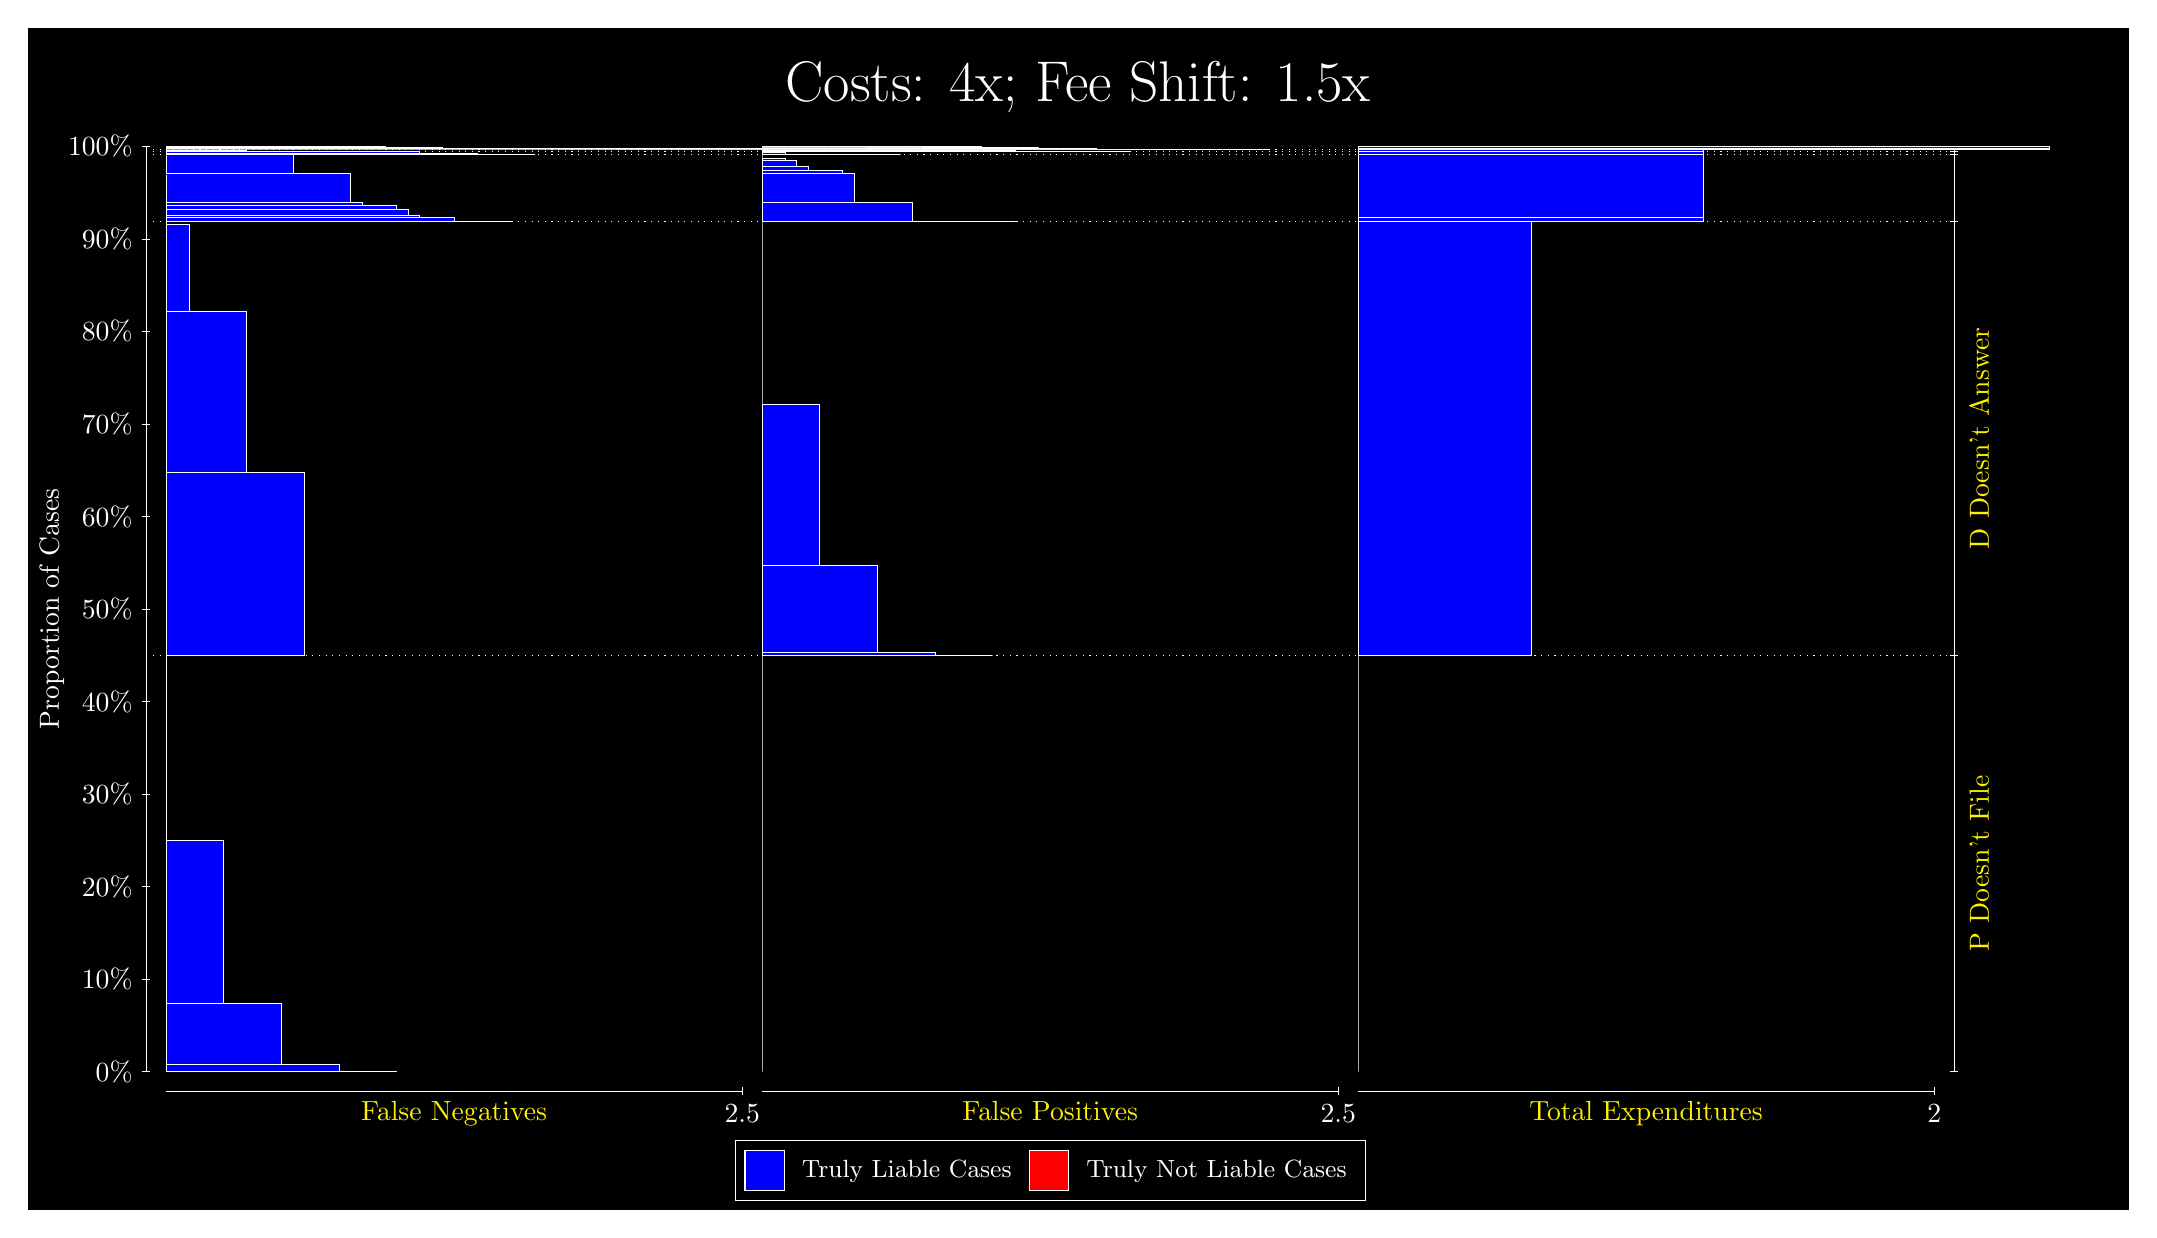
\begin{tikzpicture}
\draw[fill=black] (0,0) rectangle (26.667,15);
\draw[text=white] (0,13.5) rectangle (26.667,15) node[midway] {\huge Costs: 4x; Fee Shift: 1.5x};
\draw[white, very thin] (1.5,1.75) -- (1.5,13.5);
\node[rotate=90, text=white, anchor=center] at (0.3, 7.625) {Proportion of Cases};
\draw[white, very thin] (1.45,1.75) -- (1.55,1.75);
\node[text=white, anchor=east] at (1.45, 1.75) {0\%};
\draw[white, very thin] (1.45,2.925) -- (1.55,2.925);
\node[text=white, anchor=east] at (1.45, 2.925) {10\%};
\draw[white, very thin] (1.45,4.1) -- (1.55,4.1);
\node[text=white, anchor=east] at (1.45, 4.1) {20\%};
\draw[white, very thin] (1.45,5.275) -- (1.55,5.275);
\node[text=white, anchor=east] at (1.45, 5.275) {30\%};
\draw[white, very thin] (1.45,6.45) -- (1.55,6.45);
\node[text=white, anchor=east] at (1.45, 6.45) {40\%};
\draw[white, very thin] (1.45,7.625) -- (1.55,7.625);
\node[text=white, anchor=east] at (1.45, 7.625) {50\%};
\draw[white, very thin] (1.45,8.8) -- (1.55,8.8);
\node[text=white, anchor=east] at (1.45, 8.8) {60\%};
\draw[white, very thin] (1.45,9.975) -- (1.55,9.975);
\node[text=white, anchor=east] at (1.45, 9.975) {70\%};
\draw[white, very thin] (1.45,11.15) -- (1.55,11.15);
\node[text=white, anchor=east] at (1.45, 11.15) {80\%};
\draw[white, very thin] (1.45,12.325) -- (1.55,12.325);
\node[text=white, anchor=east] at (1.45, 12.325) {90\%};
\draw[white, very thin] (1.45,13.5) -- (1.55,13.5);
\node[text=white, anchor=east] at (1.45, 13.5) {100\%};

\draw[white, very thin] (24.457,1.75) -- (24.457,13.5);
\draw[white, very thin] (24.407,1.75) -- (24.507,1.75);
\node[anchor=west] at (24.407, 1.75) {};
\draw[white, very thin] (24.407,7.037) -- (24.507,7.037);
\node[anchor=west] at (24.407, 7.037) {};
\draw[white, very thin] (24.407,12.549) -- (24.507,12.549);
\node[anchor=west] at (24.407, 12.549) {};
\draw[white, very thin] (24.407,13.399) -- (24.507,13.399);
\node[anchor=west] at (24.407, 13.399) {};
\draw[white, very thin] (24.407,13.435) -- (24.507,13.435);
\node[anchor=west] at (24.407, 13.435) {};
\draw[white, very thin] (24.407,13.465) -- (24.507,13.465);
\node[anchor=west] at (24.407, 13.465) {};
\draw[white, very thin] (24.407,13.5) -- (24.507,13.5);
\node[anchor=west] at (24.407, 13.5) {};

\draw[white, very thin, fill=blue] (1.75,1.75) rectangle (4.6775,1.7509);
\draw[white, very thin, fill=blue] (1.75,1.7509) rectangle (3.9457,1.8467);
\draw[white, very thin, fill=blue] (1.75,1.8467) rectangle (3.2138,2.6206);
\draw[white, very thin, fill=blue] (1.75,2.6206) rectangle (2.4819,4.6898);
\draw[white, very thin, fill=red] (1.75,4.6898) rectangle (1.75,4.6898);
\draw[white, very thin, fill=blue] (1.75,4.6898) rectangle (1.75,7.037);
\draw[white, very thin, fill=blue] (1.75,7.037) rectangle (3.5065,9.3594);
\draw[white, very thin, fill=blue] (1.75,9.3594) rectangle (2.7746,11.411);
\draw[white, very thin, fill=blue] (1.75,11.411) rectangle (2.0428,12.511);
\draw[white, very thin, fill=red] (1.75,12.511) rectangle (1.75,12.511);
\draw[white, very thin, fill=blue] (1.75,12.511) rectangle (1.75,12.549);
\draw[white, very thin, fill=blue] (1.75,12.549) rectangle (6.1413,12.549);
\draw[white, very thin, fill=blue] (1.75,12.549) rectangle (5.5558,12.552);
\draw[white, very thin, fill=blue] (1.75,12.552) rectangle (5.4094,12.6);
\draw[white, very thin, fill=blue] (1.75,12.6) rectangle (4.9703,12.622);
\draw[white, very thin, fill=blue] (1.75,12.622) rectangle (4.8239,12.696);
\draw[white, very thin, fill=blue] (1.75,12.696) rectangle (4.6775,12.754);
\draw[white, very thin, fill=blue] (1.75,12.754) rectangle (4.2384,12.784);
\draw[white, very thin, fill=blue] (1.75,12.784) rectangle (4.092,13.153);
\draw[white, very thin, fill=blue] (1.75,13.153) rectangle (3.9457,13.154);
\draw[white, very thin, fill=blue] (1.75,13.154) rectangle (3.5065,13.154);
\draw[white, very thin, fill=blue] (1.75,13.154) rectangle (3.3602,13.396);
\draw[white, very thin, fill=blue] (1.75,13.396) rectangle (3.2138,13.396);
\draw[white, very thin, fill=blue] (1.75,13.396) rectangle (2.7746,13.396);
\draw[white, very thin, fill=blue] (1.75,13.396) rectangle (2.6283,13.399);
\draw[white, very thin, fill=blue] (1.75,13.399) rectangle (2.0428,13.399);
\draw[white, very thin, fill=red] (1.75,13.399) rectangle (1.75,13.399);
\draw[white, very thin, fill=blue] (1.75,13.399) rectangle (6.4341,13.399);
\draw[white, very thin, fill=blue] (1.75,13.399) rectangle (5.7022,13.415);
\draw[white, very thin, fill=blue] (1.75,13.415) rectangle (4.9703,13.435);
\draw[white, very thin, fill=blue] (1.75,13.435) rectangle (4.2384,13.435);
\draw[white, very thin, fill=blue] (1.75,13.435) rectangle (3.5065,13.435);
\draw[white, very thin, fill=red] (1.75,13.435) rectangle (1.75,13.435);
\draw[white, very thin, fill=blue] (1.75,13.435) rectangle (3.5065,13.436);
\draw[white, very thin, fill=blue] (1.75,13.436) rectangle (2.7746,13.454);
\draw[white, very thin, fill=blue] (1.75,13.454) rectangle (2.0428,13.465);
\draw[white, very thin, fill=red] (1.75,13.465) rectangle (1.75,13.465);
\draw[white, very thin, fill=blue] (1.75,13.465) rectangle (1.75,13.465);
\draw[white, very thin, fill=blue] (1.75,13.465) rectangle (13.46,13.465);
\draw[white, very thin, fill=blue] (1.75,13.465) rectangle (12.728,13.465);
\draw[white, very thin, fill=blue] (1.75,13.465) rectangle (11.996,13.466);
\draw[white, very thin, fill=blue] (1.75,13.466) rectangle (11.265,13.47);
\draw[white, very thin, fill=blue] (1.75,13.47) rectangle (10.533,13.47);
\draw[white, very thin, fill=blue] (1.75,13.47) rectangle (9.8008,13.47);
\draw[white, very thin, fill=blue] (1.75,13.47) rectangle (7.4587,13.47);
\draw[white, very thin, fill=blue] (1.75,13.47) rectangle (6.7268,13.47);
\draw[white, very thin, fill=blue] (1.75,13.47) rectangle (5.9949,13.474);
\draw[white, very thin, fill=blue] (1.75,13.474) rectangle (5.2631,13.492);
\draw[white, very thin, fill=blue] (1.75,13.492) rectangle (4.5312,13.5);
\draw[white, very thin, fill=blue] (1.75,13.5) rectangle (3.7993,13.5);
\draw[white, very thin, fill=blue] (1.75,13.5) rectangle (3.0674,13.5);
\draw[white, very thin, fill=blue] (1.75,13.5) rectangle (2.3355,13.5);
\draw[white, very thin, fill=red] (1.75,13.5) rectangle (1.75,13.5);
\draw[white, very thin, fill=red] (9.3189,1.75) rectangle (9.3189,1.75);
\draw[white, very thin, fill=blue] (9.3189,1.75) rectangle (9.3189,7.037);
\draw[white, very thin, fill=red] (9.3189,7.037) rectangle (12.246,7.037);
\draw[white, very thin, fill=blue] (9.3189,7.037) rectangle (12.246,7.037);
\draw[white, very thin, fill=blue] (9.3189,7.037) rectangle (11.515,7.0746);
\draw[white, very thin, fill=blue] (9.3189,7.0746) rectangle (10.783,8.1743);
\draw[white, very thin, fill=blue] (9.3189,8.1743) rectangle (10.051,10.226);
\draw[white, very thin, fill=blue] (9.3189,10.226) rectangle (9.3189,12.549);
\draw[white, very thin, fill=red] (9.3189,12.549) rectangle (12.539,12.549);
\draw[white, very thin, fill=blue] (9.3189,12.549) rectangle (12.539,12.549);
\draw[white, very thin, fill=red] (9.3189,12.549) rectangle (11.954,12.549);
\draw[white, very thin, fill=blue] (9.3189,12.549) rectangle (11.954,12.552);
\draw[white, very thin, fill=blue] (9.3189,12.552) rectangle (11.807,12.552);
\draw[white, very thin, fill=red] (9.3189,12.552) rectangle (11.368,12.552);
\draw[white, very thin, fill=blue] (9.3189,12.552) rectangle (11.368,12.552);
\draw[white, very thin, fill=blue] (9.3189,12.552) rectangle (11.222,12.793);
\draw[white, very thin, fill=blue] (9.3189,12.793) rectangle (11.075,12.794);
\draw[white, very thin, fill=blue] (9.3189,12.794) rectangle (10.636,12.795);
\draw[white, very thin, fill=blue] (9.3189,12.795) rectangle (10.49,13.163);
\draw[white, very thin, fill=blue] (9.3189,13.163) rectangle (10.344,13.194);
\draw[white, very thin, fill=blue] (9.3189,13.194) rectangle (9.9044,13.252);
\draw[white, very thin, fill=blue] (9.3189,13.252) rectangle (9.758,13.326);
\draw[white, very thin, fill=blue] (9.3189,13.326) rectangle (9.6116,13.348);
\draw[white, very thin, fill=blue] (9.3189,13.348) rectangle (9.3189,13.399);
\draw[white, very thin, fill=red] (9.3189,13.399) rectangle (11.075,13.399);
\draw[white, very thin, fill=blue] (9.3189,13.399) rectangle (11.075,13.399);
\draw[white, very thin, fill=blue] (9.3189,13.399) rectangle (10.344,13.399);
\draw[white, very thin, fill=blue] (9.3189,13.399) rectangle (9.6116,13.419);
\draw[white, very thin, fill=blue] (9.3189,13.419) rectangle (9.3189,13.435);
\draw[white, very thin, fill=red] (9.3189,13.435) rectangle (14.003,13.435);
\draw[white, very thin, fill=blue] (9.3189,13.435) rectangle (14.003,13.435);
\draw[white, very thin, fill=blue] (9.3189,13.435) rectangle (13.271,13.435);
\draw[white, very thin, fill=blue] (9.3189,13.435) rectangle (12.539,13.447);
\draw[white, very thin, fill=blue] (9.3189,13.447) rectangle (11.807,13.465);
\draw[white, very thin, fill=blue] (9.3189,13.465) rectangle (11.075,13.465);
\draw[white, very thin, fill=red] (9.3189,13.465) rectangle (15.759,13.465);
\draw[white, very thin, fill=blue] (9.3189,13.465) rectangle (15.759,13.465);
\draw[white, very thin, fill=blue] (9.3189,13.465) rectangle (15.028,13.465);
\draw[white, very thin, fill=red] (9.3189,13.465) rectangle (15.028,13.465);
\draw[white, very thin, fill=blue] (9.3189,13.465) rectangle (15.028,13.465);
\draw[white, very thin, fill=blue] (9.3189,13.465) rectangle (14.296,13.466);
\draw[white, very thin, fill=red] (9.3189,13.466) rectangle (14.296,13.466);
\draw[white, very thin, fill=blue] (9.3189,13.466) rectangle (14.296,13.466);
\draw[white, very thin, fill=blue] (9.3189,13.466) rectangle (13.564,13.469);
\draw[white, very thin, fill=red] (9.3189,13.469) rectangle (13.564,13.469);
\draw[white, very thin, fill=blue] (9.3189,13.469) rectangle (13.564,13.473);
\draw[white, very thin, fill=blue] (9.3189,13.473) rectangle (12.832,13.474);
\draw[white, very thin, fill=blue] (9.3189,13.474) rectangle (12.832,13.491);
\draw[white, very thin, fill=blue] (9.3189,13.491) rectangle (12.1,13.495);
\draw[white, very thin, fill=blue] (9.3189,13.495) rectangle (11.368,13.495);
\draw[white, very thin, fill=blue] (9.3189,13.495) rectangle (10.636,13.495);
\draw[white, very thin, fill=red] (9.3189,13.495) rectangle (9.3189,13.495);
\draw[white, very thin, fill=blue] (9.3189,13.495) rectangle (9.3189,13.5);
\draw[white, very thin, fill=red] (16.888,1.75) rectangle (16.888,1.75);
\draw[white, very thin, fill=blue] (16.888,1.75) rectangle (16.888,7.037);
\draw[white, very thin, fill=red] (16.888,7.037) rectangle (19.083,7.037);
\draw[white, very thin, fill=blue] (16.888,7.037) rectangle (19.083,12.549);
\draw[white, very thin, fill=red] (16.888,12.549) rectangle (21.279,12.549);
\draw[white, very thin, fill=blue] (16.888,12.549) rectangle (21.279,12.602);
\draw[white, very thin, fill=red] (16.888,12.602) rectangle (21.279,12.602);
\draw[white, very thin, fill=blue] (16.888,12.602) rectangle (21.279,13.399);
\draw[white, very thin, fill=red] (16.888,13.399) rectangle (21.279,13.399);
\draw[white, very thin, fill=blue] (16.888,13.399) rectangle (21.279,13.435);
\draw[white, very thin, fill=red] (16.888,13.435) rectangle (21.279,13.435);
\draw[white, very thin, fill=blue] (16.888,13.435) rectangle (21.279,13.465);
\draw[white, very thin, fill=red] (16.888,13.465) rectangle (25.67,13.465);
\draw[white, very thin, fill=blue] (16.888,13.465) rectangle (25.67,13.475);
\draw[white, very thin, fill=red] (16.888,13.475) rectangle (25.67,13.475);
\draw[white, very thin, fill=blue] (16.888,13.475) rectangle (25.67,13.5);
\draw[white, dotted] (1.5,7.037) -- (24.457,7.037);
\draw[white, dotted] (1.5,12.549) -- (24.457,12.549);
\draw[white, dotted] (1.5,13.399) -- (24.457,13.399);
\draw[white, dotted] (1.5,13.435) -- (24.457,13.435);
\draw[white, dotted] (1.5,13.465) -- (24.457,13.465);
\draw[white, very thin] (1.75,1.5) -- (9.0689,1.5);
\node[text=yellow, anchor=north] at (5.4094, 1.5) {False Negatives};
\draw[white, very thin] (9.0689,1.45) -- (9.0689,1.55);
\node[text=white, anchor=north] at (9.0689, 1.45) {2.5};

\draw[white, very thin] (9.3189,1.5) -- (16.638,1.5);
\node[text=yellow, anchor=north] at (12.978, 1.5) {False Positives};
\draw[white, very thin] (16.638,1.45) -- (16.638,1.55);
\node[text=white, anchor=north] at (16.638, 1.45) {2.5};

\draw[white, very thin] (16.888,1.5) -- (24.207,1.5);
\node[text=yellow, anchor=north] at (20.547, 1.5) {Total Expenditures};
\draw[white, very thin] (24.207,1.45) -- (24.207,1.55);
\node[text=white, anchor=north] at (24.207, 1.45) {2};

\node[text=yellow, centered, rotate=90] at (24.777, 4.3935) {P Doesn't File};
\node[text=yellow, centered, rotate=90] at (24.777, 9.7928) {D Doesn't Answer};





\draw (12.978300999999998,1.5) node[draw=none] (baseCoordinate) {};
\begin{scope}[align=center]
        \matrix[scale=0.5, draw=white, below=0.5cm of baseCoordinate, nodes={draw}, column sep=0.1cm]{
            \node[rectangle, draw, minimum width=0.5cm, minimum height=0.5cm, fill=blue] {}; &
            \node[draw=none, font=\small, text=white] (B) {Truly Liable Cases}; &
            \node[rectangle, draw, minimum width=0.5cm, minimum height=0.5cm, fill=red] {}; &
            \node[draw=none, font=\small, text=white] (B) {Truly Not Liable Cases}; \\
            };
\end{scope}

\end{tikzpicture}
\end{document}